\documentclass[draft,ms]{agujournal2019}
\usepackage{url} %this package should fix any errors with URLs in refs.
\usepackage{lineno}


\usepackage{amsmath}
\usepackage{setspace}
\usepackage{graphicx}
\usepackage{upgreek}
\usepackage{subcaption}
\usepackage{bm}
\usepackage{pdfpages}
\usepackage{float}
\usepackage{multirow}
\usepackage{enumitem}

\usepackage[inline]{trackchanges} %for better track changes. finalnew option will compile document with changes incorporated.
\usepackage{soul}
\linenumbers

\draftfalse


\journalname{Journal of Advances in Modeling Earth Systems (JAMES)}


\begin{document}

\title{Application of a phase-field model on snow isothermal metamorphism}


\authors{=list all authors here=}


% \affiliation{1}{First Affiliation}
% \affiliation{2}{Second Affiliation}

\affiliation{=number=}{=Affiliation Address=}

\correspondingauthor{=name=}{=email address=}

\begin{keypoints}
\item A phase-field model is applied on the curvature-driven process of equi-temperature metamorphism and used on tomographic snow microstructures.
\item The model is calibrated through the condensation coefficient parameter by fitting experimental and simulated data.
\item Equi-temperature metamorphism evolution is predicted on a representative range of snow microstructures. Microstructural and physical properties are analyzed.
\end{keypoints}


\begin{abstract}
[ enter your Abstract here ]
\end{abstract}

\section*{Plain Language Summary}
[ enter your Plain Language Summary here or delete this section]



\section{Introduction}
\label{sec:intro}
Snow on the ground is a complex material made of an ice skeleton in an air matrix that undergoes continuous transformations. Especially, snow evolves through processes of mass redistribution due to thermodynamic mechanisms called snow metamorphism. Different types of snow metamorphism take place depending on the temperature and humidity conditions as well as on the snow microstructure itself. Considering metamorphism is key as it impacts snowpack physical properties, including mechanical properties involved in avalanche processes or thermo-physical properties that drive the surface energy budget of snowpacks \cite{vionnet_detailed_2012, lehning_physical_2002}.\\

Equi-temperature metamorphism (ETM), also called isothermal metamorphism, occurs in snow in quasi-isothermal conditions and is driven by curvature gradients at the ice-air interface. Low curvature ice surfaces have a lower saturation water vapor than the high curvature ones. Those curvature gradients lead thus to gradients of saturation vapor density causing vapor transfer across the pores (diffusion and convection) as well as phase changes (sublimation and condensation). Ice sublimates on higher curvature surfaces and  water vapor deposits on lower curvature surfaces. At the grain scale, the strong concavities and convexities are replaced by rounder surfaces, and bounds are created between grains. The overall structure of snow gets rounder, coarser, and more sintered \cite{colbeck_thermodynamics_1980}. This morphological changes come together with mechanical grain rearrangement leading to snow settling. The resulting type of snow is referred to as rounded grains (RG) by The International Classification for Seasonal Snow on the Ground \cite{fierz2009international}. Equi-temperature metamorphism is constantly taking place in snow but at different levels of intensity. The higher the contrast in curvature and the higher the snow temperature, the more active the equi-temperature metamorphism. In the presence of high temperature gradients, the influence of curvature effects becomes insignificant as the effect of the temperature gradient metamorphism (TGM) predominates.\\

Modeling the physical processes of metamorphism at fine scale requires the  description of the snow microstructure and its evolution (moving interfaces) as well as water vapor transport across the microstructure. Different degrees of approximation can be used: kinetic dynamics at the interface i.e. considering instantaneous diffusion in the pores ; kinetics dynamics and diffusion are considered ; kinetics, diffusion and settling are modeled. Moreover, models can be applied on simplified geometry, as in  \citeA{miller_microstructural_2003} who considered a 2D regular network of spherical grains, or on real snow microstructure, taking as inputs 3D images of elementary representative volume of snow obtained from microtomography ($\upmu$CT). \citeA{flin_full_2003} considered fully curvature-driven snow metamorphism based on the kinetic limited assumption, and simulated it with an iterative method on 3D tomographic images. Comparisons between modeled and experimental microstructures is also shown. \citeA{vetter_simulating_2010} used a Monte-Carlo algorithm to simulate the isothermal metamorphism with the kinetic limited assumption and implemented a simple gravity model to account for settling. They obtained consistent results with observations although the model rely on experimental fitting.\\
Recently, phase-field models have been developed to handle the numerical costs and complexity \cite{kaempfer_phase-field_2009, granger_physique_2019, bretin_phase-field_2019}. \citeA{kaempfer_phase-field_2009} suggested a phase-field model for snow metamorphism considering interface kinetics and diffusion. \citeA{kaempfer_phase-field_2009} were pioneers with the phase-field method applied to snow metamorphism, and their results are consistent with observations. However, evaluations are qualitative and limited only on one temperature gradient case, mainly because of the numerical cost of the model. 
\citeA{bretin_phase-field_2019} developed a very efficient phase-field multi-grain growth model and applied it to curvature-driven interface evolution, which could be relevant for equi-temperature snow metamorphism but has only been applied to simplified geometry.\\
To this day, a phase-field snow model enables the best efficiency and accuracy, but modeling snow growth relies on a choice of the condensation parameter $\alpha$. This parameter embodies the surface physics that governs how water molecules are incorporated into the ice lattice and is thus key to model metamorphism. The $\alpha$ coefficient ranges from 0 to 1. One can think of $\alpha$ as a sticking probability, equal to the probability that a water vapor molecule striking the ice surface becomes assimilated into the crystal lattice. However, it is still poorly understood and quantified, notably because of its complex dependencies to temperature, humidity and crystalline orientation. Numerous values can be found in the literature, ranging from 10$^{-3}$ to 10$^{-1}$ \cite<e.g.,>{libbrecht_measurements_2013}. The large uncertainty on this coefficient was one of the main limiting parameter for metamorphism models accuracy.\\
In this article we attend to go further by applying the phase-field growth model of \citeA{bretin_phase-field_2019} on the curvature-driven snow equi-temperature metamorphism usable on $\upmu$CT images. We calibrated the model by finding a single value of the condensation coefficient using an experimental equi-temperature series. This calibration have been evaluated on an independent ETM series. The model have been used to predict ETM on a representative range of 3D microstructures. Those results are shown along with microstructural properties and transport properties, which are analyzed and compared to current models and parameterizations. 

\section{Method}
\label{sec:method}

\subsection{Model}
\label{subsec:model}
\begin{figure}
    \centering
    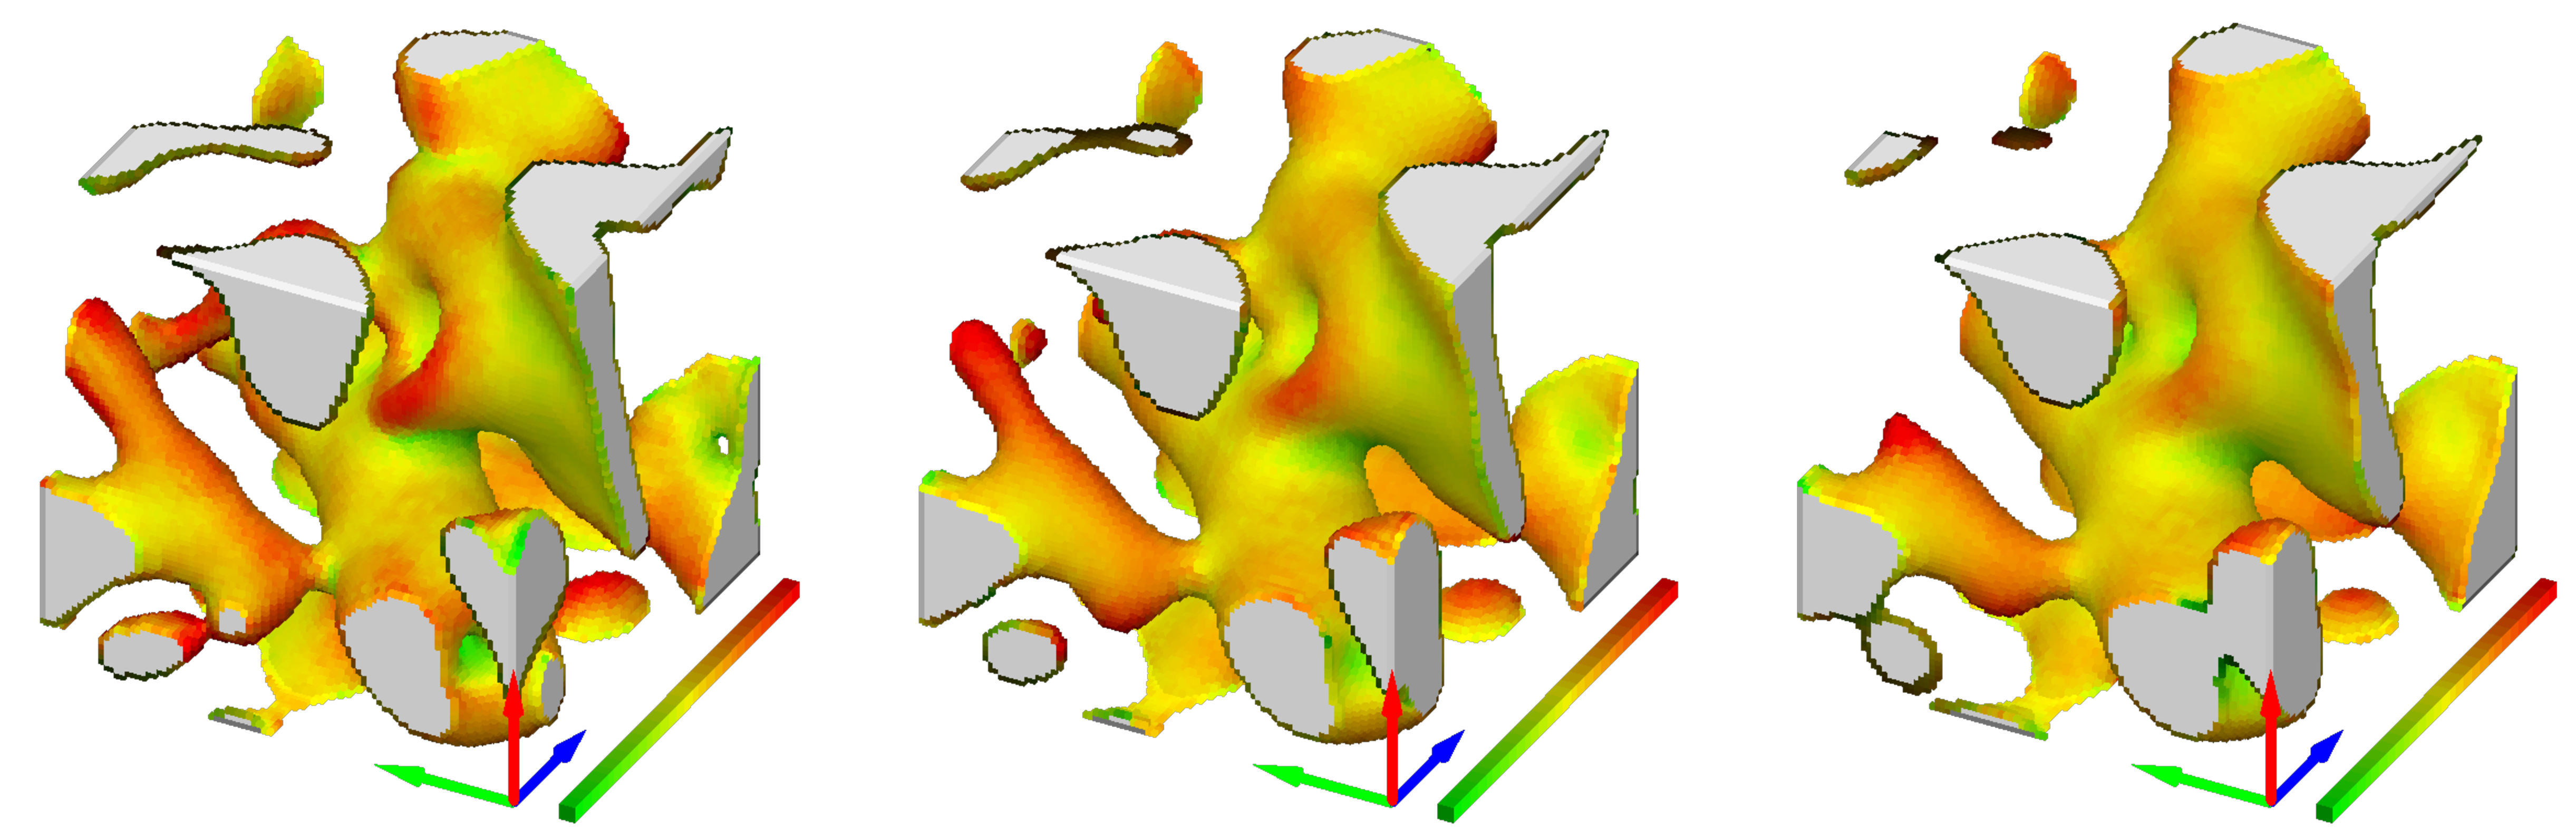
\includegraphics[width=\linewidth]{Figures/eboni_sous_volumes_simu.pdf}
    \caption{Curvature map of a three-dimensional representation of a sample evolution from \protect\citeA{hagenmuller_motion_2019} under the equi-temperature metamorphism model Snow-3D after 0, 8 and 16 days at -2$^\circ$C.}
    \label{fig:eboni_sous_volume}
\end{figure}

The model simulates the evolution of a 3D image under isothermal metamorphism. It can take as input tomographic snow samples as in Figure \ref{fig:eboni_sous_volume}. It describes the process of sublimation and deposition at the ice/air interface due to water vapor density variations driven by curvature. Vapor transport in the pore space by diffusion or convection is not simulated and is assumed to be instantaneous, so the evolution is limited by the kinetics at the interface. Finally, the model does not include any mechanics and the settling of the ice grains is thus not described here.\\

The metamorphism is considered here to be fully curvature-driven and the temperature is isotropic and constant. The variations of vapor density with curvature can be described by Kelvin's Law:
\begin{equation}\rho_v(C)=\rho_v^{\mathrm{ref}}(T) \exp \left(\frac{2 \gamma \Omega C}{R T}\right)\end{equation}
\noindent with $\rho_v(C)$ the vapor density at a point of mean curvature $C$ in m$^{-1}$, $R$ the universal gas constant in J K$^{-1}$ mol$^{-1}$, $T$ the temperature of snow in K and $\rho_v^{\mathrm{ref}}$ in kg m$^{-3}$ the vapor density at equilibrium with a flat ice surface at temperature $T$. $\Omega$ is the molar volume of ice in m$^3$ mol$^{-1}$ and $\gamma$ is the surface tension between ice and vapor in N m$^{-1}$. 
The vapor density gradient induced by curvature differences results in ice sublimation on high curvature surfaces and deposition of water vapor on low curvature surfaces, leading to rounding, coarsening and sintering the ice structure. In Figure \ref{fig:eboni_sous_volume} the effect of sublimation-deposition is shown with concave surfaces in green and convex surfaces in red \cite{ogawa2006representation}. Generally $(2 \gamma \Omega C / R T) \ll 1$, we can thus write:

\begin{equation}
\Delta \rho_v=\rho_v - \rho_v^{\mathrm{ref}} \simeq \rho_v^{\mathrm{ref}}(T)\left(\frac{2 \gamma \Omega C}{R T}\right)\label{eq:kelv_lin} 
\end{equation}

This equation gives us access to the saturation vapor density distribution within pores depending on the surrounding interface curvatures. Using the Hertz-Knudsen equation, it can be linked to the growth speed of the interfaces.

\begin{align}
v_{n} &= \alpha v_{k i n} \sigma(T, C) \\
v_{k i n} &= \frac{\rho_{v s}(T, C)}{\rho_i}\sqrt{\frac{R T}{2 \pi M}} \\
\sigma(T, C) &= \frac{\rho_v - \rho_{v s}(T, C)}{\rho_{v s}(T, C)}
\end{align}
\label{eq:hertz_knu}

This equation defines the kinetic velocity $v_{\mathrm{kin}}$. $M$ is the molar mass of a water molecule in kg mol$^{-1}$, $\alpha$ is the condensation coefficient, $\rho_i$ is the ice density, $\sigma$ is the local supersaturation, and $\rho_{v s}$ is the water vapor density at saturation. The saturation density above a flat surface $\rho_{v}^{\mathrm{ref}}$ has been largely studied, and can be determined using one of the existing parameterizations. We choose here to use \citeA{gofflow} parameterization that seems to be largely used in our range of temperature. 

%phase-field
To model the micro-scale, it is important to model the snow slab as multiple grains with their own dynamics, interacting with each others. The physical phenomenon studied here occurs at the interface between grains and air in the pores, and is driven by the geometry of this interface. This model uses the phase-field description to model the sublimation-deposition process. This method can solve coupled heat and mass transfer, with topological changes. The idea is to avoid the explicit interfaces problem by introducing the phase-field, a function that varies smoothly from a value in ice to another value in air. It results in a system of partial equations much easier to handle numerically \cite{bretin_and_denis_discrete-continuous_2015, kaempfer_phase-field_2009}.

\begin{figure}
    \centering
    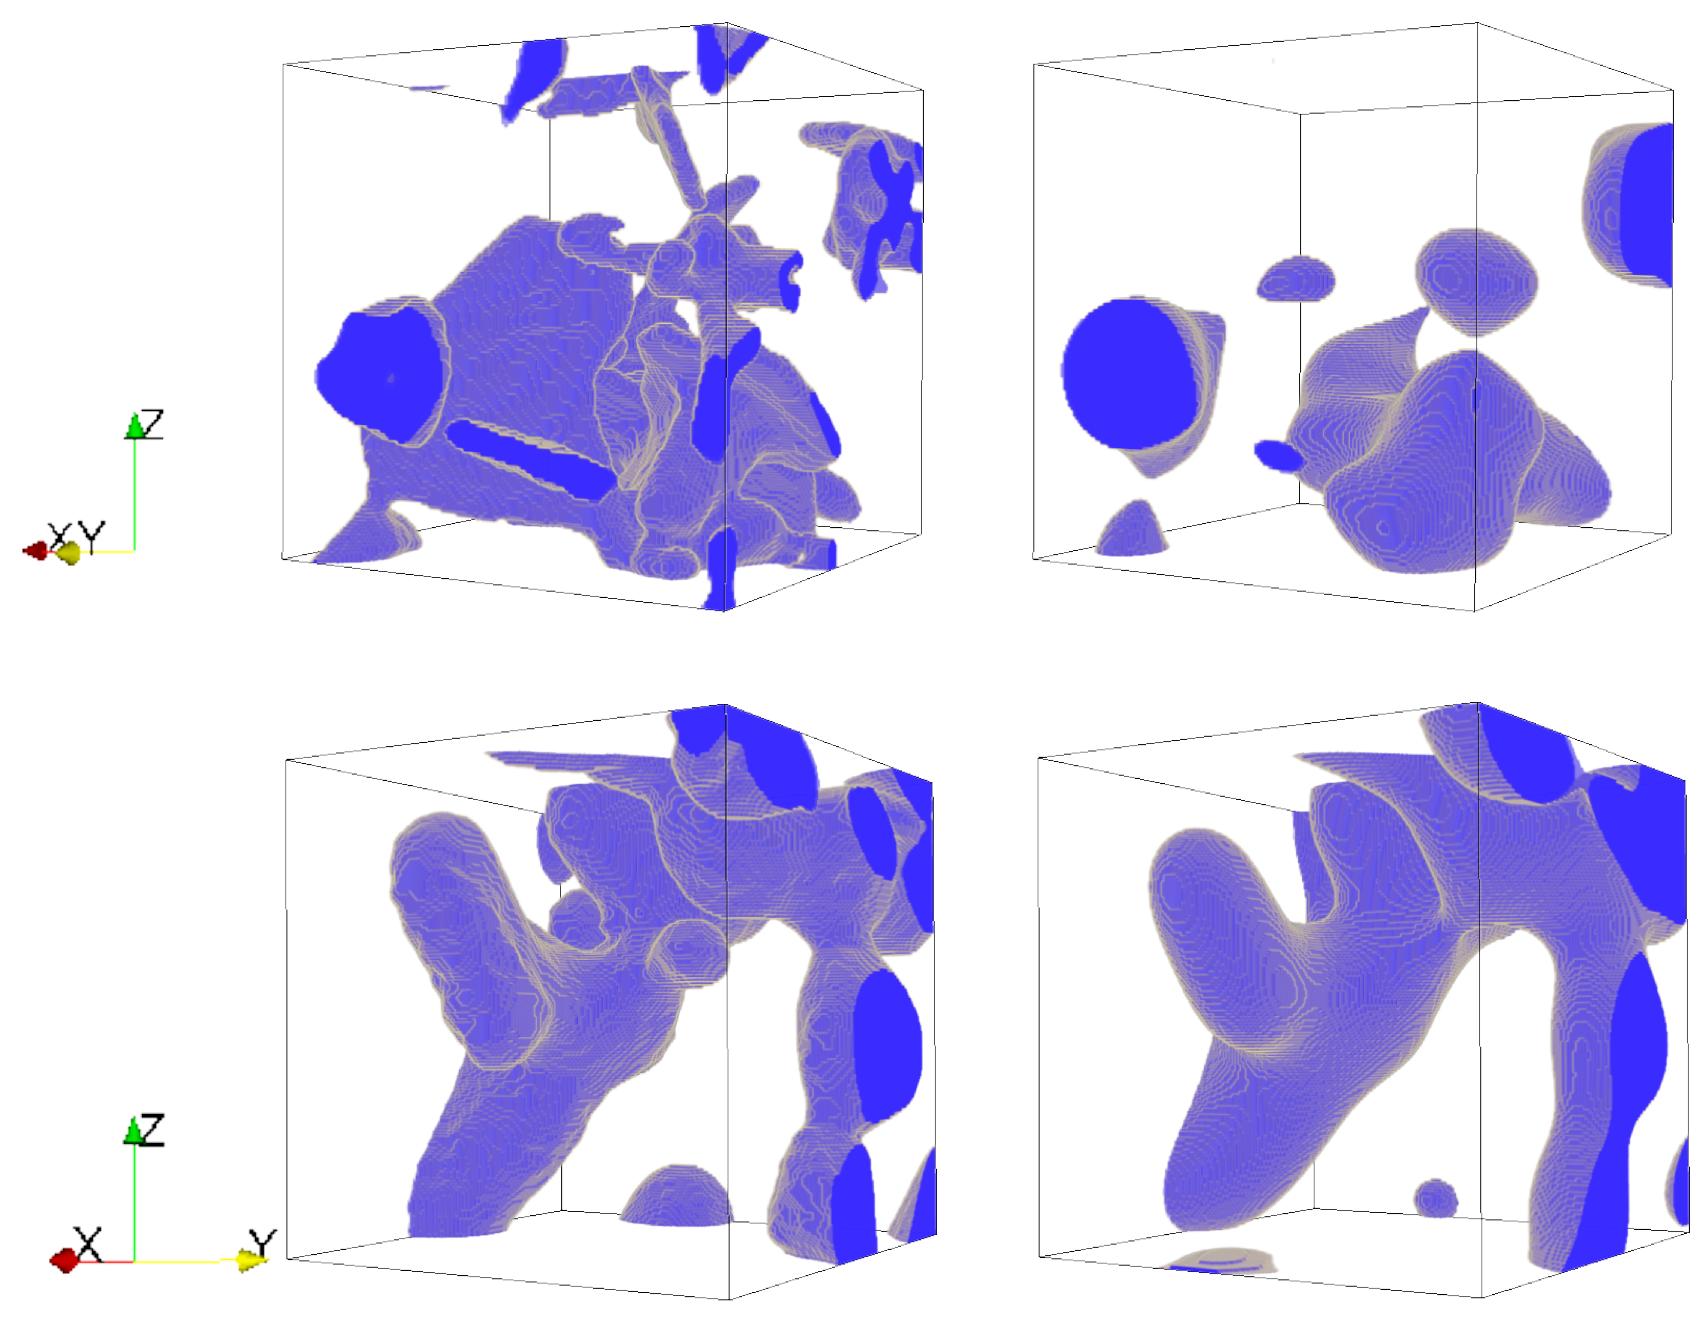
\includegraphics[width=0.7\linewidth]{Figures/disconnections_iso01_iso15.pdf}
    \caption{Influence of the starting snow type on the disconnections. a) Fresh snow from \protect\cite{flin_three-dimensional_2004} series: initial state (left) and after 40 days of simulation (right) ; b) Sample that underwent 30 days of isothermal conditions: initial state (left) and after 40 days of simulation (right) }
    \label{fig:disco}
\end{figure}

The model takes as input a binary 3D image of a snow sample digitized with X-ray absorption microtomography. The adjustable parameters are the time step $t_{step}$ and the number of time steps $n$. The output is a series of 3D binary images that underwent the simulated isothermal metamorphism. Artefacts are induced by the sample geometry during the simulation, including: 
\begin{itemize}[label=-]

\item Edge effect: The driver of the model is the curvature difference. Due to the periodic boundary conditions of the model, some curvature misestimations may occur at the edge of snow 3D volumes, i.e., snow grains may be considered as cut by the borders of the image, leading to very high curvatures. To avoid those errors  in this area of the sample, we chose to cut a certain width (at least one heterogeneity using the covariance length $l_c$(Sec. \ref{subsec:methode_physical_appli})) of the image edges on the simulation outputs before the calculation of the microstructural properties.\\
\vspace{0.2cm}

\item Grain disconnection: As the model does not simulate gravity, when particles are disconnected because of morphological evolution, they tend to ``float" in the air phase before getting small enough to disappear. The consequence is that the model gives realistic results only when the input snow image is not too porous and fresh. To prevent this non physical phenomenon, we suppress disconnected ice particles during the simulation, and we chose as inputs snow samples that already underwent preliminary stages of metamorphism. An example of disconnections is shown in Figure \ref{fig:disco}. 
% As an example, we loose 6.10$^{-4}$ g of Grad3 sample (0.08 g) during the simulated 75 days of ETM with the suppression of disconnected particles. 
\end{itemize}

\begin{table}[ht]
\hspace*{-0.5cm}
\begin{tabular}{|c|c|c|c|c|c|}
\hline Reference & ETM stage & Resolution & Dimension & Density & Snow types \\
 &  & ($\mu$m) &(voxels) & (kg m$^{-3}$) &  \\
\hline 
\cite{flin_three-dimensional_2004} & $2026\ \mathrm{h}$, T = $-2^{\circ} \mathrm{C}$ & 4.9 & 512 & 158 & \small{$\mathrm{PP} \rightarrow \mathrm{RG}$} \\
\cite{hagenmuller_motion_2019} & 4 days, $\mathrm{T}=-2^{\circ} \mathrm{C}$ & 7.5 & 450 & 212 & \small{$\mathrm{DF/RG}$} \\
\hline
\end{tabular}
\caption{Experimental equi-temperature series used to calibrate and evaluate the model. The density is the initial density of the used portion of each series. The snow types separated by an arrow present the initial and final type of the series.}
\label{tab:series_exp}
\end{table}


\begin{table}[ht]
\hspace*{-3cm}
\begin{tabular}{|c|c|c|c|c|c|}
\hline Name (Reference) & Metamorphism stage & Resolution & Dimension & Density & Snow types \\
 &  & ($\upmu$m) &(voxels) & (kg m$^{-3}$) &  \\
\hline 
I17 \small{\cite{dumont2017experimental}} & Recent snow & 7.3 & 700 & 147 & \small{$\mathrm{DF}$} \\
TG2 \small{\cite{dumont2017experimental}} & 16 days, $\mathrm{TG}=19\ \mathrm{K}\ \mathrm{m}^{-1}, \mathrm{T}=-5^{\circ} \mathrm{C}$ & 7 & 700 & 254 & \small{$\mathrm{FC} / \mathrm{DH}$} \\
Grad3 \small{\cite{flin2011computations}} & 8 days, $\mathrm{TG}=100\ \mathrm{K}\ \mathrm{m}^{-1}, \mathrm{T}=-5^{\circ} \mathrm{C}$ & 10 & 600 & 372 & \small{$\mathrm{DH}$} \\
7G9m \small{\cite{calonne_study_2014}} & 21 days, $\mathrm{TG}=43\ \mathrm{K}\ \mathrm{m}^{-1}, \mathrm{T}=-4^{\circ} \mathrm{C}$ & 9.7 & 950 & 314 & \small{$\mathrm{DH}$} \\
\hline
\end{tabular}
\caption{Experimental images used as prediction to simulate isothermal metamorphism.}
\label{tab:series_sim}
\end{table}

\subsection{Calibration} 
\label{subsec:calib}

An important effort has been made in calibrating the model through the condensation coefficient $\alpha$. In our case, finding $\alpha$ is equivalent to scale the simulation steps to real time steps via the equations \cite{bretin_and_denis_discrete-continuous_2015}: \\

\begin{subequations}\label{equ:alpha}
\begin{minipage}{0.45\textwidth}\begin{align}
    t_\varphi = \frac{t_{\text{sim}} \rho_i dx^2}{\alpha \rho_{v s}(T) d_0} \sqrt{\frac{2 \pi M}{R T}}
\end{align}\end{minipage}
\begin{minipage}{0.45\textwidth}\begin{align}\label{equ:d0}
    d_0 = \frac{\lambda a^3}{k T}
\end{align}\end{minipage}
\end{subequations}\\
\vspace{0.3cm}

\noindent with $t_{\varphi}$ the physical time in s, $t_{\text{sim}}$ the simulated time in the model, $dx$ the image resolution in m. Equation (\ref{equ:d0}) comes from the  Gibbs-Thomson relation and links the capillary length $d_0$ to $\lambda$ the interfacial free energy in J m$^{-2}$ and $a$ the mean intermolecular spacing in the ice in m \cite{kaempfer_phase-field_2009}. The saturation vapor density $\rho_{\text{sat}}$ has been deduced as a function of temperature with the formulation of \citeA{gofflow}.% which is generally considered as the reference equation \cite{murphy2005review}. 

To calibrate the model we used the experimental series of \citeA{flin_three-dimensional_2004} (cf Table \ref{tab:series_exp}). This series is a 3 months long experiment of isothermal metamorphism at -2$^\circ$C that lead to 10 tomographic images. From this series we only use the samples from 118 h to the end of the experiment. We chose to set the first images aside to avoid problems with the primary stage of settling. We removed on each side of the image a layer with a thickness equal to the size of two heterogeneities (0.6 mm) to avoid edge artifacts. With this transformation the volumes were still in the range of the representative elementary volumes (REV). The calibration process is schematized in 5 steps in Figure \ref{fig:workflow}. For each selected image of the experimental series: \\
\begin{enumerate}
    \item We used the model Snow-3D to obtain a simulated series composed of 10 images. 
    \item We calculated the SSA evolution of the series during the simulation (Graphs b) and c)).
    \item We fitted the simulated SSA to the experimental SSA curve (Graph a)) by adjusting the x-axis. More precisely, we scaled the simulation steps to the real time (Equation \ref{equ:alpha}) such that they match the experiment best by minimizing the Root Mean Square Error (RMSE) between the two curves.   
    \item We used the simulation time and the fitted physical time to find a value of the condensation coefficient $\alpha$ (Equation \ref{equ:alpha}). A weighted average is calculated on $\alpha$ using the inverse of the RMSE as weight to maximize the influence of the $\alpha$ originating from the best fit to the experimental curve. 
\end{enumerate}

\hspace*{-0.2cm}
\begin{figure}
    \centering
    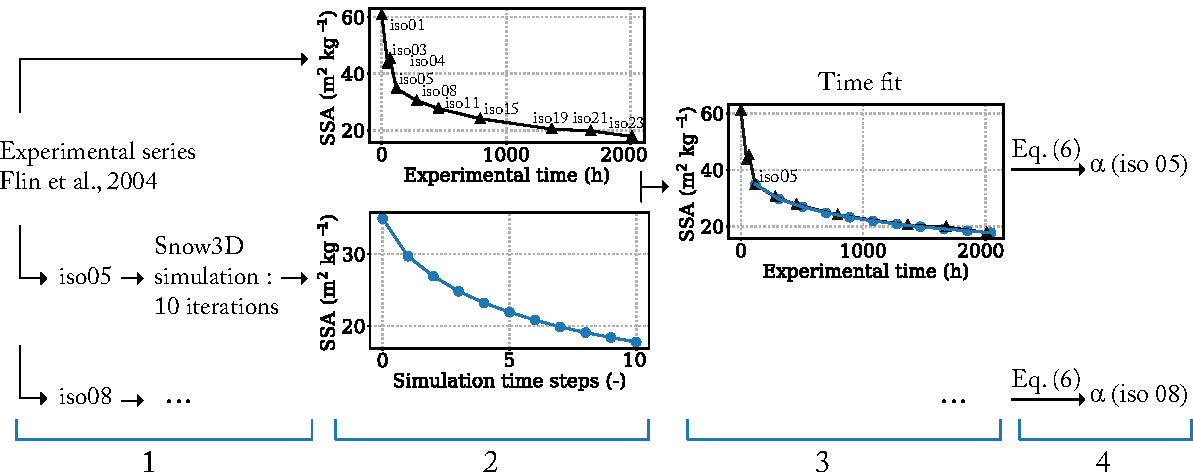
\includegraphics[width = \linewidth]{Figures/workflow_aff.pdf}
    \caption{Workflow of the time calibration approach}
    \label{fig:workflow}
\end{figure}
Those steps have been applied to each images of the experimental series, from 5 days to 33 days. The three last images of the experimental series are not used because of the lack of data to fit them with. It results in 7 simulated series composed of 10 images simulating equi-temperature metamorphism from a different input image, i.e. from a different metamorphism stage. The condensation coefficient $\alpha$ have been calibrated using the SSA parameter because it is a good indicator of the global sample microstructure evolution. The resulting condensation coefficient is $\alpha = ( 9.9 \pm 0.6) 10^{-4}$. As the temperature condition of \citeA{flin_three-dimensional_2004} is -2$^\circ$C, the calibrated model can only be used to simulate ETM at -2$^\circ$C. The uncertainty is calculated using a classical propagation of uncertainties of $\alpha$ through the equation (\ref{equ:alpha}). To see the influence of $\alpha$ in the microstructural parameters, we calculated the variation of the microstructural parameters as a function of $\alpha$ variation. In the range of our $\alpha$ variation through the different samples, the parameters such as density, specific surface area and covariance length (described in Section \ref{subsec:methode_physical_appli}) only have a maximum alteration of 5\%, which is small compared to the precision of those parameters. 

\subsection{ETM model prediction: computation of snow properties}
\label{subsec:methode_physical_appli}
Once the model calibration through the condensation coefficient $\alpha$ have been performed, we evaluated the calibrated model using the independent ETM series of \citeA{hagenmuller_motion_2019} (Table \ref{tab:series_exp}). The series of \citeA{hagenmuller_motion_2019} is a 110h long experiment of isothermal metamorphism at -2$^\circ$C with 32 tomographic images. The series was used to study dust particles in snow under temperature gradient conditions. As our model does not work on more than 2 phases, the dust particles were converted to air before using it in Snow-3D. A temperature gradient of 5 K m$^{-1}$ was detected and corrected after 38h of experiment, thus we only work with the final part of the series (approx. 70h of isothermal metamorphism). In \citeA{hagenmuller_motion_2019} the snow sample was observed with operando X-ray tomography, meaning than the same sample was scanned at regular interval. In contrast, the \citeA{flin_three-dimensional_2004} series uses samples that were extruded at different locations of the snow slab for each tomographic scan.\\

After considering the calibration evaluation and validation, the model was used to predict equi-temperature metamorphism effects on different experimental images (Table \ref{tab:series_sim}). Those samples have been chosen to constitute a representative range of snow microstructures. We ran the simulations with Snow-3D taking 4 different snow samples as initial stage, named I17 (DF), TG2 (FC/DH), Grad3 (DH), and 7G9m (DH) (see table \ref{tab:series_sim}). The simulations were performed with isothermal conditions at a temperature T = -2$^\circ$C and $\alpha = 9.9\ 10^{-4}$. It led to 4 series of 4 to 11 images simulating from 70 days to 80 days of isothermal metamorphism. This time range enables to capture the important physical evolution while remaining realistic. In Figure \ref{fig:evolutions_3D}, we see the simulated series of our 4 samples, with a perspective view of three steps for each series, and vertical slices associated to those steps.\\

To characterize our simulated and experimental microstructures, we calculated on our volumes a range of microstructural and physical properties. Those properties are defined and used as in \citeA{calonne_study_2014}.

\noindent \textbf{Microstructural properties}$\quad$ To describe the microstructure of our snow images, we computed microstructural properties on the volumes using counting and normal vectors algorithms. The properties used are:
\begin{itemize}

    \item The mean curvature MC (mm$^{-1}$), defined as $\mathrm{MC} = \left(C_{min} + C_{max})\right/2$ with $C_{min}$ and $C_{max}$ respectively the minimum and maximum 2-D curvatures at one point of the surface. As those values are computed for each point of the surface, they are represented as statistical distributions. Values near 0 mm$^{-1}$ correspond to flat surfaces, positive values are convex surfaces, and negative MC are concave surfaces; the higher the values, the more concave or convex the surfaces \cite{flin_three-dimensional_2004, brzoska2007using, wang2012curvature}. 
    % In the Figure \ref{fig:MC} in both histograms the mean decreases towards 0 with iterations, which corresponds to larger and rounded grains. In the downward mean curvature, the asymmetry at the first iterations is explained by the facets (plane surfaces) oriented downward from the TG metamorphism that will get rounder with the isothermal metamorphism model.\\
    
    \item The porosity $\phi$ (-), computed with a simple voxel counting algorithm. Snow density $\rho_{\mathrm{s}}$ is linked to the porosity  by $\rho_{\mathrm{s}}=\rho_{\mathrm{i}}(1-\phi)$ with $\rho_{\mathrm{i}}=917\ \mathrm{kg\ m^{-3}}$ the ice density.
 
    \item The specific surface area SSA (m$^2$ kg$^{-1}$), is defined by the ratio between the total ice surface of a sample and its volume of ice per mass unit: $\mathrm{SSA}=S/V \times \rho_{i}$ \cite{flin2011computations, berryman1998planar}.
    
    \item  The covariance (or correlation) length $l_{c}$, calculated along the x-, y-and z- direction of the images, provides a characteristic length of the microstructure, corresponding to the characteristic size of heterogeneities. It is used to characterize the basic microstructure geometry \cite{lowe2013general}. 
    
    \item Anisotropy coefficient
    $\mathcal{A}(\star)$, that can be computed for each microstructural and physical property that are computed along 3 dimensions. This coefficient is defined as the ratio between the vertical component over the horizontal one, such as $\mathcal{A}(\star)=\star_{z} / \star x y$. The property is considered isotropic if it exhibits a coefficient close to 1, otherwise the property is anisotropic. For example, $\mathcal{A}(l_c)$ largely above 1 means that the covariance length is higher in the vertical direction than in the horizontal one, and thus describe a structure that is vertically elongated.
\end{itemize}

% \noindent \textbf{Physical properties}$\quad$ To further characterise our 3D images, we also analyzed  the effective thermal conductivity tensor $\mathbf{k}\mathrm{^{eff}}$, the effective coefficient of water vapor diffusion tensor $\mathbf{D}\mathrm{^{eff}}$ and the effective air permeability tensor $\mathbf{K}\mathrm{^{eff}}$, which are the key properties involved in snow metamorphism. Properties were computed on our 3D images with the software Geodict (http://www.geodict.de) that uses the finite difference method. For each property, a specific boundary value problem, arising from a homogenization technique \cite{auriault2009homogenization, calonne2015macroscopic}, is solved on the images applying periodic boundary conditions on the external boundaries of each volume. \\

% \begin{itemize}
% \item The numerical estimate of heat conduction is expressed as : $\dot{q}=-\mathbf{k}\mathrm{^{eff}}\ \mathbf{grad}\ T$ at 271 K  with $\dot{q}$ (W m$^{-2}$) the heat flux and $T$ (K) the temperature using $\kappa_{air}$ = 0.024 W m$^{-1}$ K$^{-1}$, $\kappa_{ice}$ = 2.107 W m$^{-1}$ K$^{-1}$ the air and ice conductivities \cite{calonne_numerical_2011}.\\

% \vspace{0.5cm}

% \item The tortuosity tensors of the air phase $\bm{\tau}_a$ is obtained by solving the same above boundary problem as the thermal one assuming that $\kappa_{air}$ = 1 and $\kappa_{ice}$ = 0. For snow, air tortuosity is linked to the effective diffusion tensor for the water vapor by $\mathbf{D}\mathrm{^{eff}}=\phi D_{\mathrm{m}} \tau_{\mathrm{a}}$ where $D_{\mathrm{m}}\left(\text { in } \mathrm{m}^{2}\  \mathrm{s}^{-1}\right)$ is the molecular diffusion coefficient of the vapor in air at the pore scale \cite{calonne_3D_2012, calonne_study_2014}.\\
% \vspace{0.5cm}

% \item At the macro scale, the flow within the snow pores is characterized by the permeability solved with Darcy’s law: $u = -\mathbf{K}\mathrm{^{eff}} \mathbf{grad} P /\mu $
% where $\mathbf{K}\mathrm{^{eff}}$ (m$^2$) is the effective permeability, $u$ (m s$^{-1}$) is the mean velocity, $P$ (Pa) is the pressure, and $\mu$ (Pa s) is the dynamic viscosity. Because the dimension of the permeability is a square length, $\mathbf{K}\mathrm{^{eff}}$ is often normalized by a characteristic length to the square. We use the equivalent sphere radius $r_{\mathrm{es}}=3/(\mathrm{SSA} \times \rho_{\mathrm{i}})$ to introduce a dimensionless tensor: $\mathbf{K}\mathrm{^{eff*}} = \mathbf{K}\mathrm{^{eff}}/r_{\mathrm{es}}^2$  \cite{calonne_3D_2012}. \\
% \end{itemize}

% In the following, the non-diagonal terms of the tensors $\mathbf{k}\mathrm{^{eff}}$, $\mathbf{D}\mathrm{^{eff}}$ and $\mathbf{K}\mathrm{^{eff}}$ , about 50 times lower than
% diagonal terms, are not presented (the x-, y- and z-axes of 3D images correspond to the
% principal directions of the microstructure, z being along the direction of the gravity). In the following, we mostly use the vertical component, the average of the two horizontal components, and the average value of the three components of the tensors, respectively.

% --- (modifié) ----------------------------------------------------------------------------

\noindent \textbf{Physical properties}$\quad$ The 3D tensor of the effective coefficient of diffusion  $\mathbf{D}$ (m$^2$ s$^{-1}$), of the effective thermal conductivity tensor $\mathbf{k}$ and of the intrinsic permeability  $\mathbf{K}$ (m$^2$) were computed on the set of simulated 3D images. For each property, a specific boundary value problem, arising from a homogenization technique \cite{auriault2009homogenization, calonne2015macroscopic}, is solved on the images applying periodic boundary conditions on the external boundaries of each volume using the software Geodict \cite{thoemen_3d_2008}. The effective diffusion coefficient was computed with an artificial diffusion coefficient of gas in free air set to $D^{\mathrm{air}} =$ 1 m$^2$ s$^{-1}$. In this study, we present the normalized values of the effective diffusion $\mathbf{D} / D^{\mathrm{air}}$ (dimensionless). %These normalized values can be multiplied by the diffusion coefficient of the gas of interest in free air to get the physical, non-normalized values of effective diffusion coefficient of this gas in snow or firn (for example, the diffusion coefficient of vapor in free air, that is $2.036 \times 10^{-5}$ m$^2$ s$^{-1}$ at -10$^\circ$C \cite{massman_review_1998}, could be used to get the effective diffusion coefficient of vapor). 
$\mathbf{K}$ is normalized by the equivalent sphere radius $r_{\mathrm{es}}=3/(\mathrm{SSA} \times \rho_{\mathrm{i}})$ to introduce a dimensionless tensor: $\mathbf{K}\mathrm{^{*}} = \mathbf{K}/r_{\mathrm{es}}^2$  \cite{calonne_3D_2012}.
As the non-diagonal terms of the tensor $\mathbf{D}$, $\mathbf{k}$ and  $\mathbf{K}$ are negligible, we consider only the diagonal terms, i.e. seen as the eigenvalues of the tensors (the image axes $x$, $y$ and $z$ are the principal directions of the microstructure, $z$ being along the direction of gravity). Besides, the tensors are transversely isotropic as the components in $x$ are very similar to the ones in $y$.
In the following, $D$, $k$ and $K$ refer to the averages of the diagonal terms of $\mathbf{D}$, $\mathbf{k}$ and $\mathbf{K}$, respectively. $D_z$, $k_z$ and $K_z$ refer to the vertical components and $D_{xy}$, $k_{xy}$ and $K_{xy}$ refer to the mean horizontal components where $D_{xy} = (D_{x} + D_{y}) /2$, $k_{xy} = (k_{x} + k_{y}) /2$ and $K_{xy} = (K_{x} + K_{y}) /2$. Finally, the anisotropy of the properties is characterized based on the anisotropy ratio $\mathcal{A}(D) = D_z / D_{xy}$, $\mathcal{A}(k) = k_z / k_{xy}$ and $\mathcal{A}(K) = K_z / K_{xy}$ \cite<e.g.>{calonne_study_2014}.

% ------------------------------------------------------------------------------------


\section{Results}

\subsection{Model evaluation against experimental data}
\label{Section:Calibration}

\begin{figure}
    \centering
    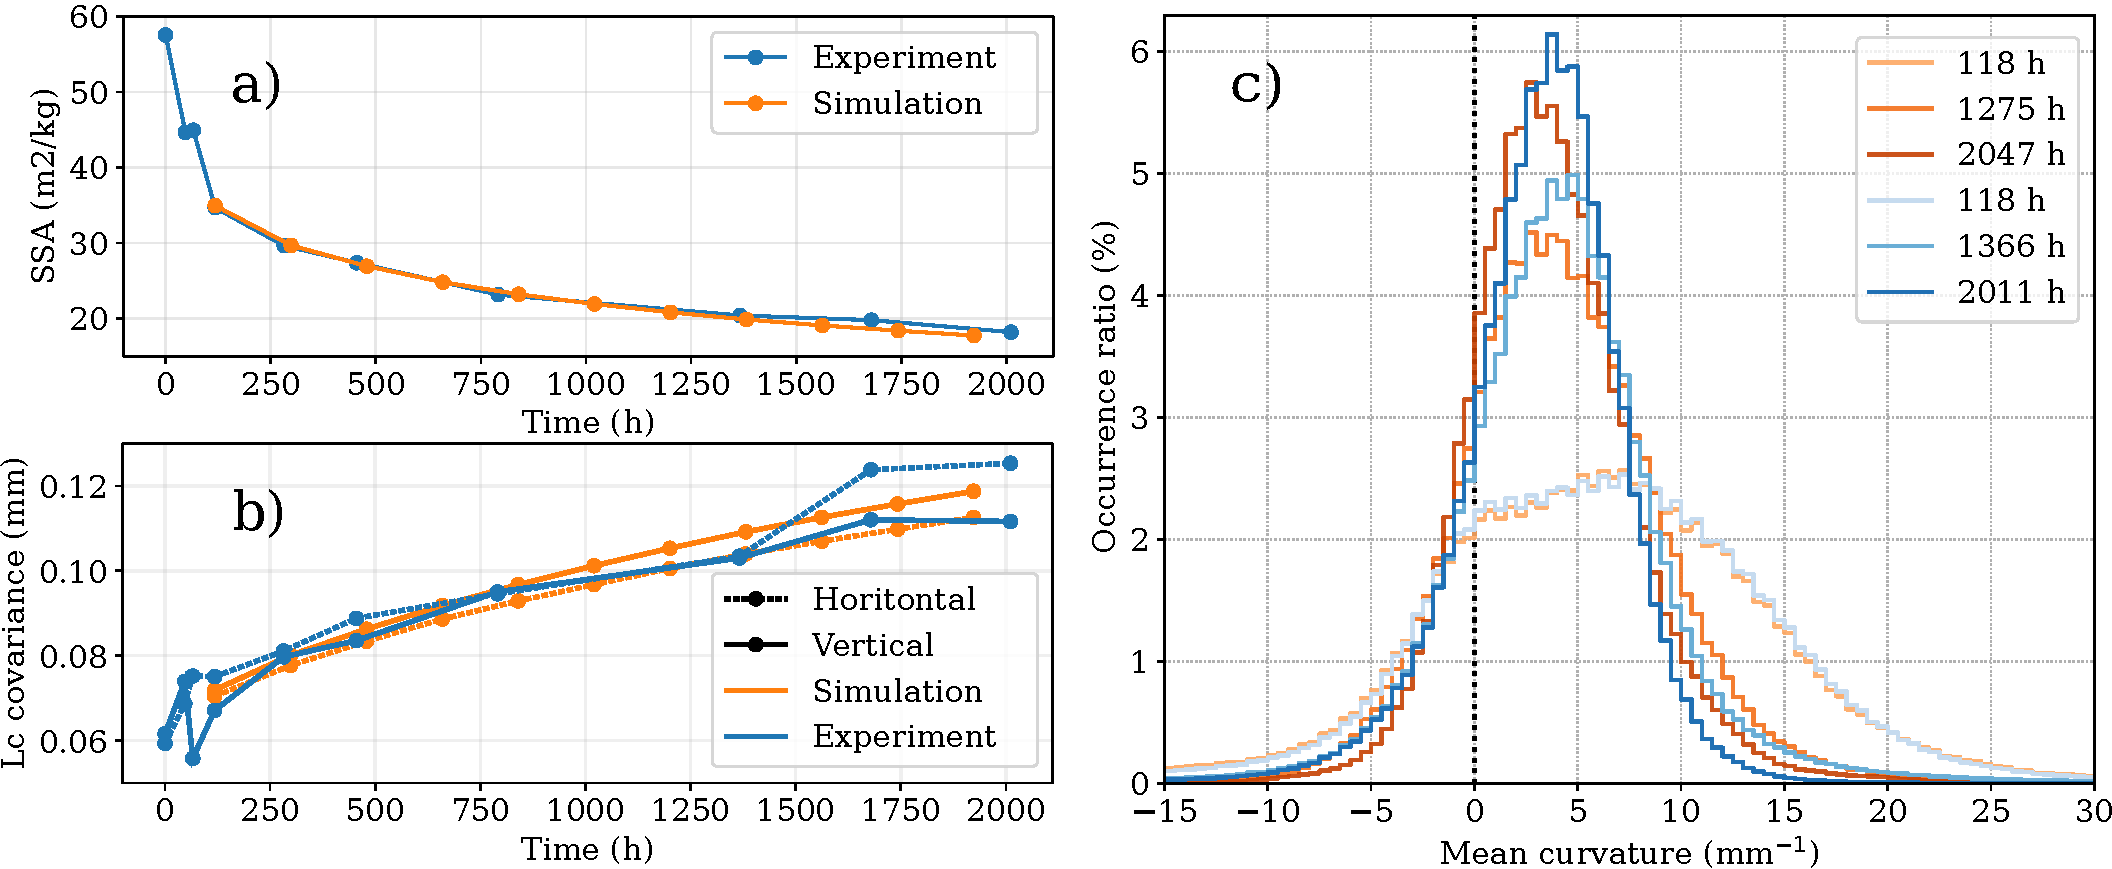
\includegraphics[width=\linewidth]{Figures/flin_evaluation_courbes_lc_ssa_histo.pdf}
    \caption{Comparison between \protect\citeA{flin_three-dimensional_2004} experimental series from the iso05 sample and simulation results. a) SSA ; b) correlation length ; c) mean curvature histograms.}
    \label{fig:flin_evaluation}
\end{figure}

% The condensation coefficient $\alpha$ have been calibrated to the experimental series of \citeA{flin_three-dimensional_2004} using the SSA parameter. In this section we test the reliability of the calibration, by comparing experimental and simulated microstructural parameters such as the SSA, the covariance length and the mean curvature. As a first step we observe the parameters concordance between experimental and simulated results for \citeA{flin_three-dimensional_2004}. Secondly, we use the independent experimental series of  \citeA{hagenmuller_motion_2019} to evaluate the calibration by looking at the same parameters.\\
% Figures \ref{fig:flin_evaluation}.a and \ref{fig:flin_evaluation}.b display the evolution of SSA, covariance length with time from the experiments and simulations, starting from the iso05 sample taken after 118h of equi-temperature conditions.
% From Figure \ref{fig:flin_evaluation}.a, we can observe that simulations follow closely the SSA decrease reported in the experiment. %This is the comparison $\alpha$ was calibrated to, it therefor has very good fit with a RMSE of $0.58\ \mathrm{m}^2\ \mathrm{kg}^{-1}$.
% The RMSE between those data is of $0.58\ \mathrm{m}^2\ \mathrm{kg}^{-1}$. We see in Figure \ref{fig:flin_evaluation}.b that the covariance length evolution in vertical and horizontal directions is well represented by the model with a small RMSE of $0.005\ \mathrm{mm}$. In Figure \ref{fig:flin_evaluation}.c mean curvature distribution presents a more detailed description of the snow microstructure in term of shape and grain size. We see the distributions are narrowing while keeping a positive mean curvature. It depicts that ice surfaces are getting more uniform towards round but less convex surfaces. The evolution of the experimental and simulated data are very similar, and we see a good agreement in the time steps.\\
% Next, Figure \ref{fig:eboni} allows evaluating our simulations against the dataset of \citeA{hagenmuller_motion_2019}. In contrast with the dataset from \citeA{flin_three-dimensional_2004}, from which we calibrated the model, this one allows independent comparisons. In Figure \ref{fig:eboni}.a, the SSA comparison reveals an overall good agreement: even if the rate of SSA decrease seems to be slightly  underestimated in the model, as shown by the deviations between model and experience towards the end of the evolution (difference of $1.47\ \mathrm{m}^2\ \mathrm{kg}^{-1}$ at 80 h), the agreement is good with a RMSE of $0.79\ \mathrm{m}^2\ \mathrm{kg}^{-1}$. In addition, the covariance length Figure \ref{fig:eboni}.b shows an even better concordance with a mean RMSE of $0.0003\ \mathrm{mm}$. In Figure \ref{fig:eboni}.c, for the mean curvature distribution the first time steps are similar between the model and the simulation, but this parameter has more variability for this series than the previous one because the time period is short and the snow grains are still small.


 Here, we evaluate the calibrated model by comparing experiments and simulations through SSA, covariance length and mean curvature.
We compared with the time series of \citeA{flin_three-dimensional_2004}, the dataset used to calibrate the condensation coefficient required in the model (Sec. \ref{subsec:calib}), as well as with the one of \citeA{hagenmuller_motion_2019} to allow for an independent comparison. Results for each time series are shown in Figure \ref{fig:flin_evaluation} and \ref{fig:eboni}, respectively. For the comparison with the data of \citeA{flin_three-dimensional_2004}, iso05, the first image used for the calibration which is a RG sample of snow scanned after 118 h of ETM, was used as initial image. \\

As expected, simulations follow closely the SSA decrease reported in the experiment of \citeA{flin_three-dimensional_2004} (Fig \ref{fig:flin_evaluation}.a).
The RMSE is of $0.58\ \mathrm{m}^2\ \mathrm{kg}^{-1}$ for SSA values evolving from 35 to 18 m$^2$ kg$^{-1}$.
Covariance lengths increase over time from around 0.07 to 0.12 mm. This overall evolution is well reproduced by the model with a small RMSE of $0.005\ \mathrm{mm}$ (Fig. \ref{fig:flin_evaluation}.b). Looking in more details, the snow microstructure gets slightly elongated in the horizontal direction with covariance length about 0.02 mm higher in the horizontal direction than in the vertical one. This is not captured in the simulations in which differences between the lengths in both directions remains rather constant over time and do not exceed 0.005 mm. We should however keep in mind that the experimental data do not only reflect a time evolution but also the spatial variability of the snow layer monitored in \citeA{flin_three-dimensional_2004}, the latter being not considered in simulations, as explained in Section \ref{sec:method}. This might explain the small disagreement observed in correlation lengths.
Finally, the mean curvature distribution presented in Figure \ref{fig:flin_evaluation}.c allows to qualitatively compare the evolution of grain surface morphology. We see the distributions are narrowing and shift toward lower mean curvature values, especially in the first time period. This depicts that ice surfaces are getting more uniform towards larger rounded grains. The evolution of the experimental and simulated data are very similar, with a good agreement at each time steps.\\

 Over the 70 hours used from the \citeA{hagenmuller_motion_2019} experiment, changes are more subtle. SSA decreases from 33 to 28 m$^2$ kg$^{-1}$, whereas correlation length increases from 0.077 to 0.087 mm in the horizontal direction and from 0.065 to 0.072 mm in the vertical one. The model performs well for the SSA with a RMSE of $0.79\ \mathrm{m}^2\ \mathrm{kg}^{-1}$ and, even better for the covariance length with a RSME of $0.0003\ \mathrm{mm}$ (mean for both directions).
The rate of SSA decrease seems however slightly underestimated by the model, reaching a difference of $1.47\ \mathrm{m}^2\ \mathrm{kg}^{-1}$ after 80 h; this is still small with respect to the SSA value range.
Overall good agreements are found for the mean curvature distribution (Fig. \ref{fig:eboni}.c). \\


% The condensation coefficient $\alpha$ have been calibrated using the SSA parameter, that is a good indicator of the global sample microstructure evolution. Others global microstructural parameters are useful to describe the snow sample, such as the covariance length and the anisotropy of covariance. The mean curvature distribution gives a more detailed description of the structure. Split between the downward facing and the upward facing distributions, this variable shows the distribution of rounded or facetted grains found depending on the orientation. The curvature is the main driver parameter of the model. The microstructural parameters of \citeA{flin_three-dimensional_2004} are shown in Figure \ref{fig:flin_evaluation} and the mean curvature distribution is shown in Figure \ref{fig:histo_flin_evaluation}.

\begin{figure}
    \centering
    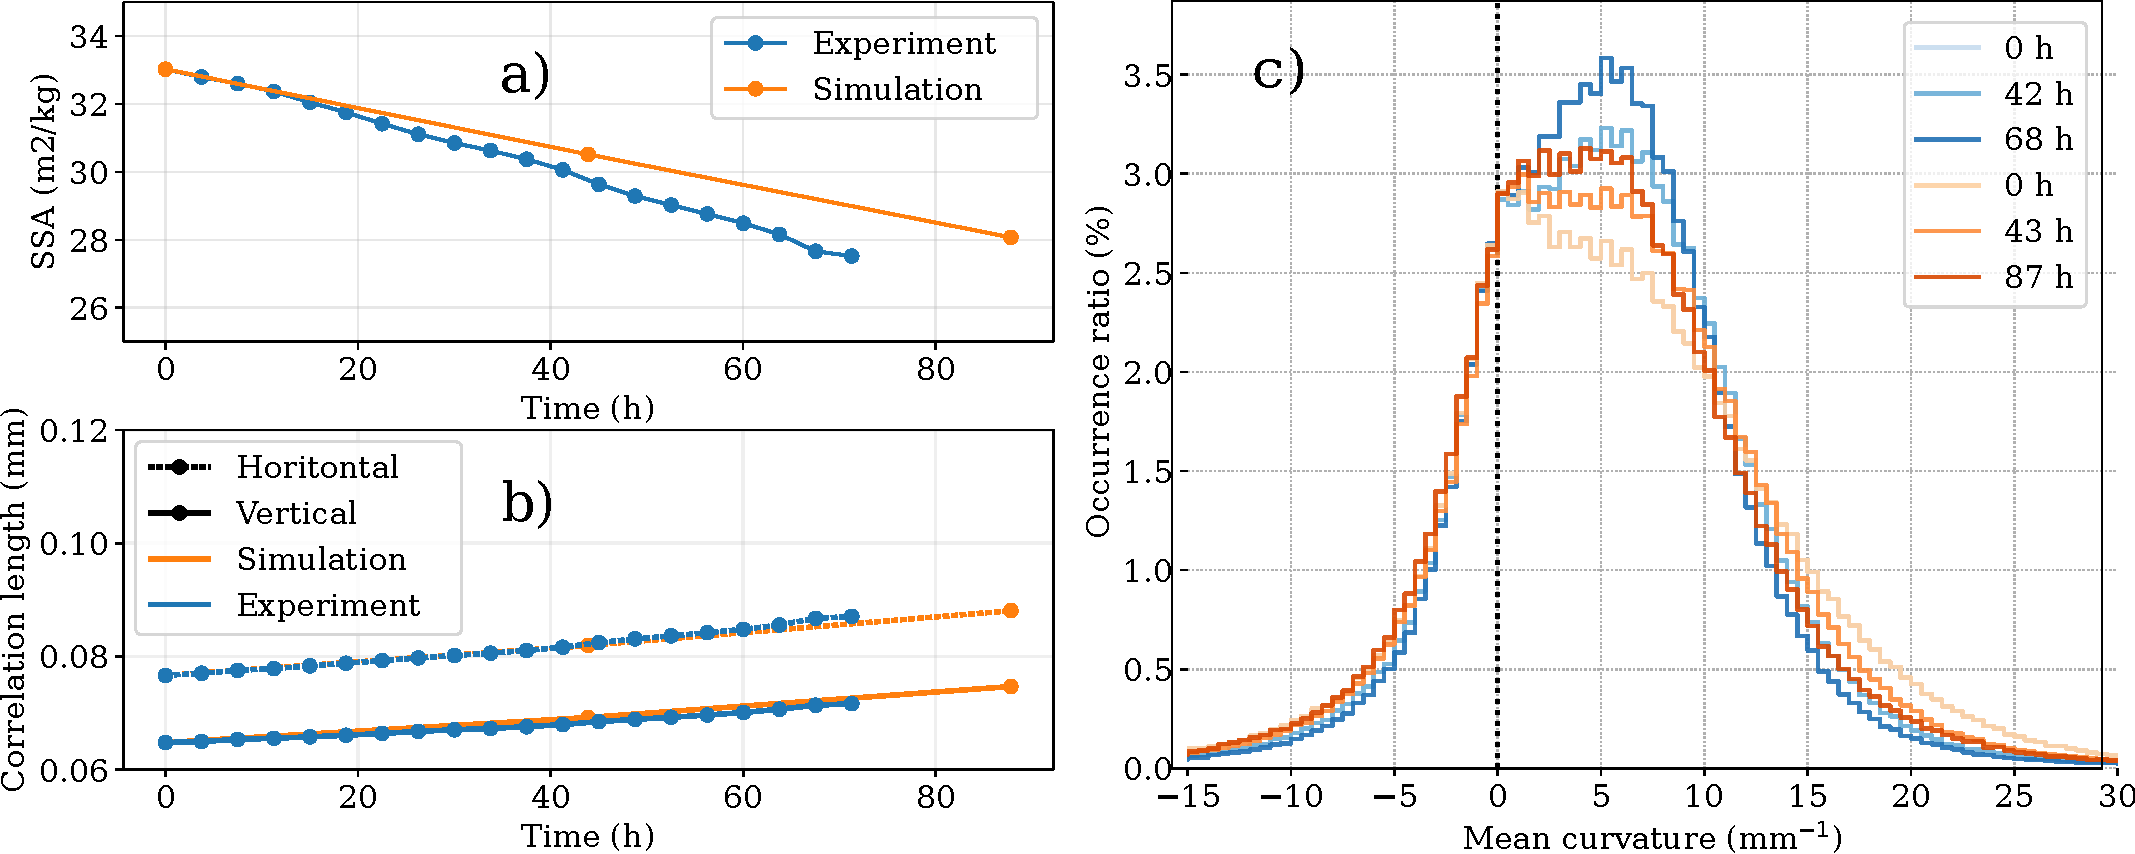
\includegraphics[width=\linewidth]{Figures/eboni_courbes_lc_ssa_histo.pdf}
    \caption{Comparison between \protect\citeA{hagenmuller_motion_2019} experimental series and simulation results. a) SSA ; b) correlation length ; c) mean curvature histograms.}
    \label{fig:eboni}
\end{figure}


\subsection{Model application: evolution of different snow microstructures during ETM}
\begin{figure}
    \centering
    \includegraphics[width =\linewidth]{Figures/evolution_3D_new_textepetit_courr.pdf}
    \caption{Simulated evolution 3D views and their vertical slices taken at the center of each cubes.}
    \label{fig:evolutions_3D}
\end{figure}
\subsubsection{Microstructural parameters}

In Figure \ref{fig:histo_i17_grad3}, we see the mean curvature distribution evolution for I17 and Grad3 samples. They are expressed in terms of occurrence ratio, which gives the percentage of the ice surface area that exhibits a mean curvature located in a particular curvature class. Those plots exhibit the driving process of the model, and give a detailed microstructure description.\\
For I17 simulated evolution (Figure \ref{fig:histo_i17_grad3}.a), the initial upward and downward distributions are similar with a peak of mean curvature located around 4 mm$^{-1}$ and an occurrence ratio of 5 \%. It shows that this sample was initially isotropic. With time, the area-averaged mean curvature decreases gradually, and the distributions are narrowing as the ice structure tend to become larger and more uniform.\\
For Grad3 evolution (Figure \ref{fig:histo_i17_grad3}.b), the initial upward and downward distributions are wider than for I17 initial sample. It can be explained by the strong concave and convex shapes encountered in Grad3 and not in I17 that already presents rounded shapes. For Grad3, the initial upward and downward surfaces exhibit clearly distinct distributions: the peak of mean curvature is located around 0 mm$^{-1}$ for the upward ones, and at 1.5 mm$^{-1}$ for the downward ones. The near 0 upward distribution depicts the plane surfaces that are typically found when looking upward a depth hoar structure unlike the downward outlook that present more concave shapes. With time, the area-averaged mean curvature stays very low but the distributions are narrowing ( approx. 7 \% occurrence ratio), showing the same trend as I17.\\


Figure \ref{fig:4_images_microstruct} shows the microstructural parameters of our 4 simulated series. For the SSA graph, we see an exponential decrease for each image, which matches with ETM experiments and similar models \cite{vetter_simulating_2010, kaempfer_observation_2007}. Each series shows different decreasing rate and shape, ranging from Grad3 with an exponential decrease of 23.7 to 9.2 m$^2$ kg$^{-1}$ to the almost linear slope of I17 curve from 20.6 to 13.7 m$^2$ kg$^{-1}$. This difference in decrease rate  is due to the initial microstructure. Grad3 shows a high initial SSA value, with sharp edges and facets that evolve quickly under isothermal conditions, unlike the sample I17 that presents rounded shapes in its initial stage.
The covariance length evolution shows the characteristic increase of the ETM, reflecting the growth of snow grains and pores \cite{lowe2011interfacial, calonne_study_2014}. Different evolution rates are again observed, from an increase of 0.05 mm for I17 to 0.09 mm for Grad3. Finally, looking at the anisotropy ratio evolution provides surprising results. The samples I17 and TG2 presenting a rather isotropic structure, with ratio close to 1, show no changes over time. Samples initially anisotropic, however, show an increase of their anisotropy, as Grad3 increasing from 1.44 to 1.62 through the simulation and, in a lesser way, 7G9m ranging from 1.24 to 1.27. By the end of the simulations, Grad3 covariance length is about two times larger in the vertical direction than in the horizontal direction. This increase in anisotropy can also be seen in the slices and 3D images : the initial vertically elongated structure is strengthening with the growing of vertical columns. This is a result of interest because one could think that a sample presenting a strong anisotropy would tend to lose it for the benefit of a more isotropic structure under the effect of a long equi-temperature exposure.

\begin{figure}
    \centering
    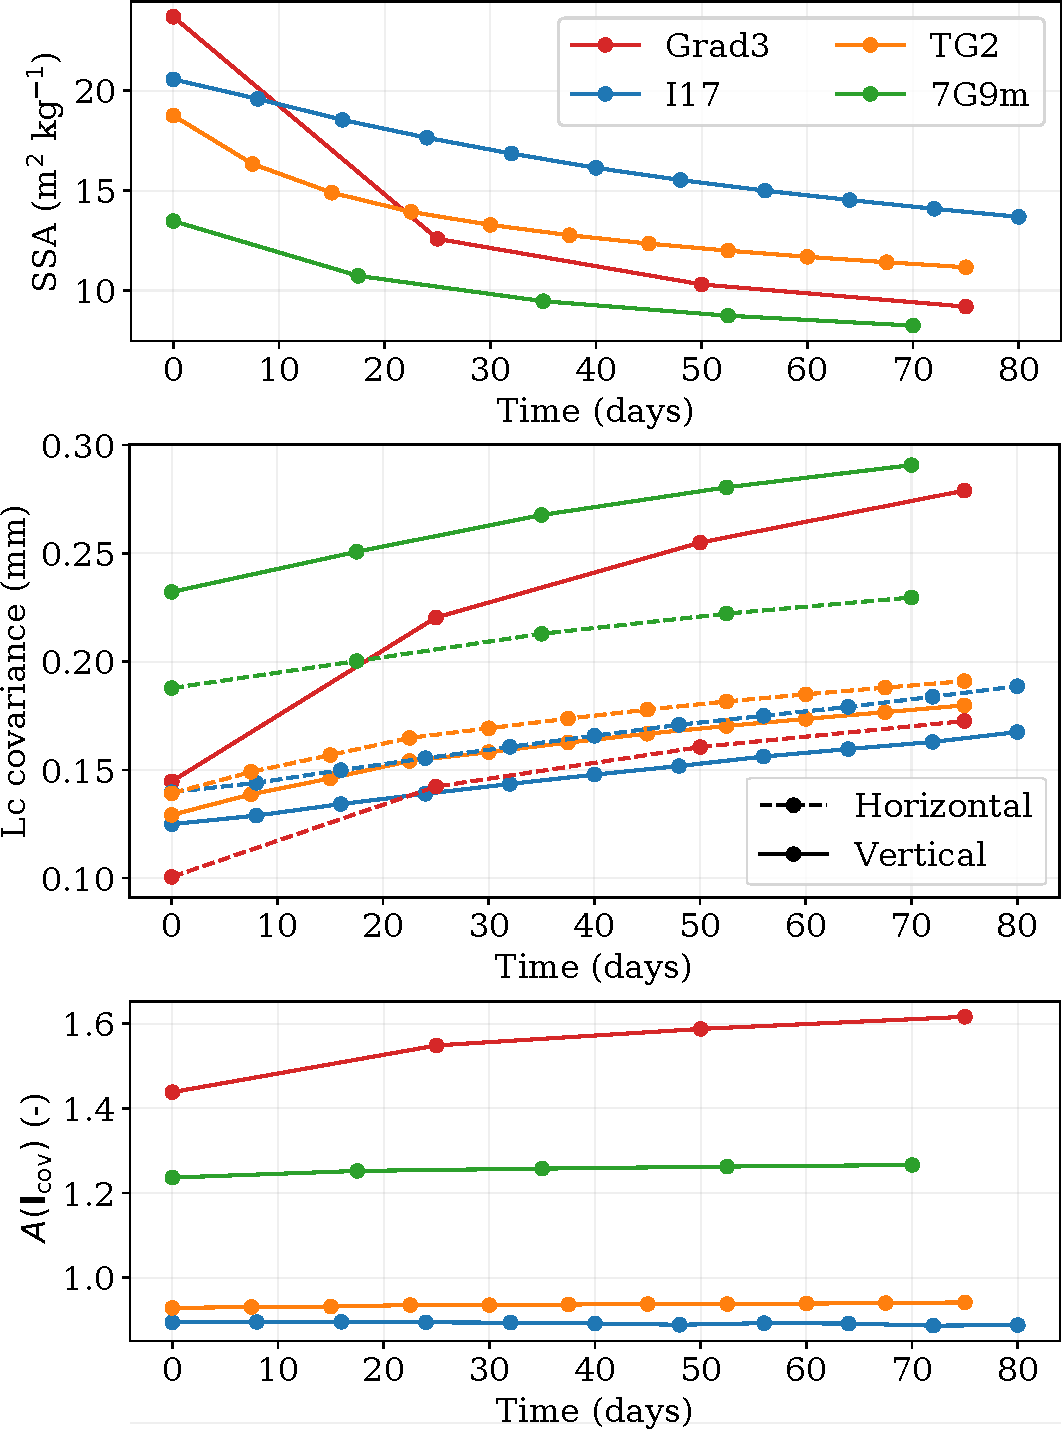
\includegraphics[width=0.6\linewidth]{Figures/4_images_microstructure.pdf}
    \caption{Microstructural parameters of the simulated series.}
    \label{fig:4_images_microstruct}
\end{figure}

\begin{figure}
    \centering
    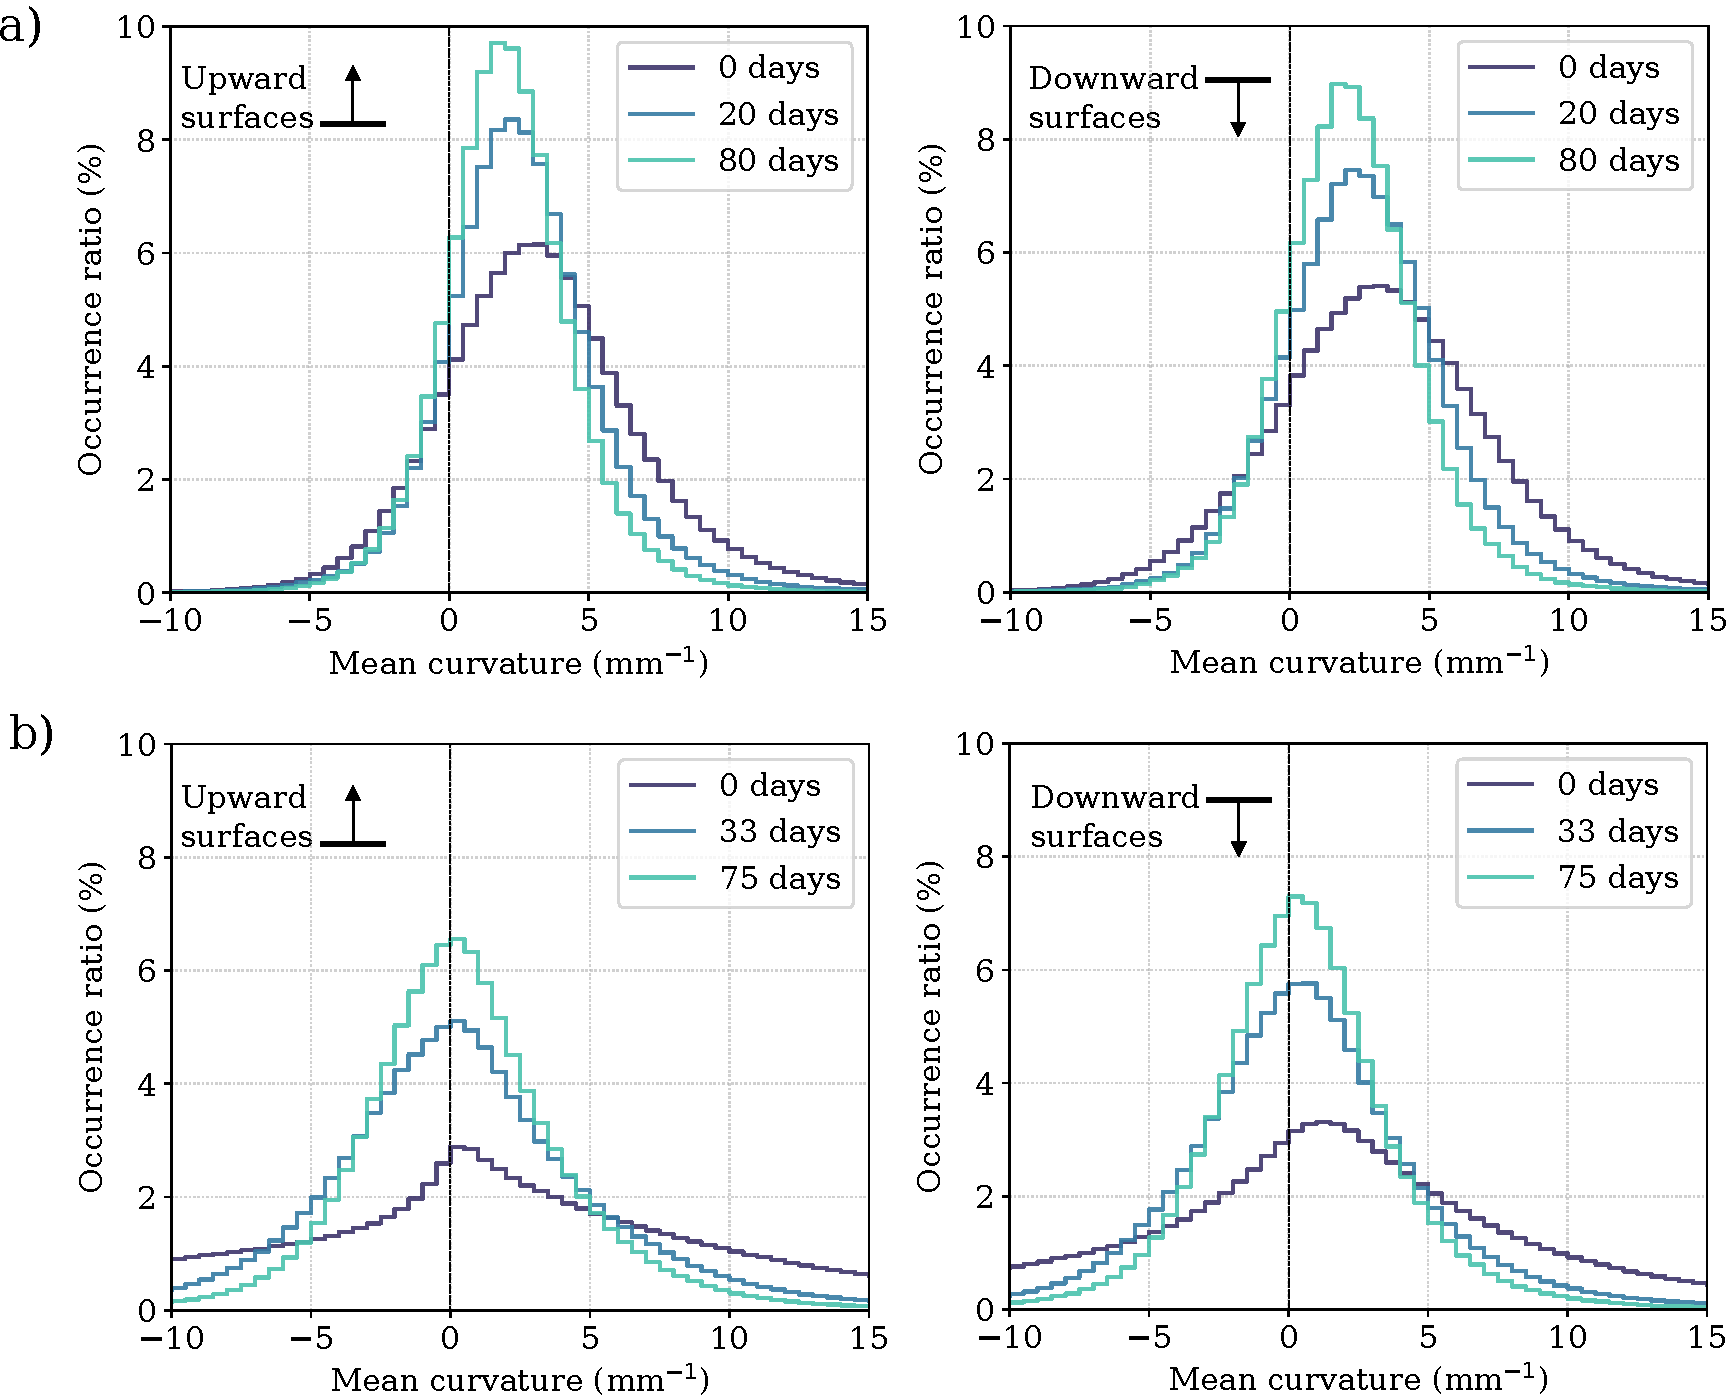
\includegraphics[width=\linewidth]{Figures/histo_i17_grad3.pdf}
    \caption{Time evolution of the mean curvature distribution from the upward (left) and downward (right) surfaces of I17 (a) and Grad3 (b) simulated series. Each curvature class is 0.5 mm$^{-1}$ wide.}
    \label{fig:histo_i17_grad3}
\end{figure}

\subsubsection{Macroscale physical properties}

Here we compare estimates of thermal conductivity, effective coefficient of diffusion, and permeability calculated on the simulated 3D images (Sec. \ref{subsec:methode_physical_appli}) with models based on simplified microstructures and current parameterizations. In Figure \ref{fig:Tplot}, conductivity, diffusivity and permeability are plotted as a function of the porosity. To show the structural anisotropy of the samples, the tips and horizontal bars of the ``T" markers represent respectively the vertical and horizontal components. Colors correspond to the ICSSG \cite{fierz2009international}.\\
 
 For the thermal conductivity, the fit of \citeA{calonne_numerical_2011} was used. This regression has been obtained using images of snow spanning a wide range of seasonal snow types using the same analysis tools we used above. It is expressed as:
\begin{equation}k_{\mathrm{th}}=2.5 \times 10^{-6} \rho_{\mathrm{s}}^{2}-1.23 \times 10^{-4} \rho_{\mathrm{s}}+0.024\end{equation}
with $\rho_{\mathrm{s}}$ the snow density, linked to the porosity by $\rho_s = (1 - \phi)\rho_i$ with $\rho_i$ the ice density.
The parameterization is in good agreement with our results and the errors are mostly linked to the anisotropy. Indeed, the vertical component of conductivity of faceted crystals and depth hoar samples like TG2, Grad3 and 7G9m is always larger than the horizontal component, while rounded grains like I17 exhibit the inverse behavior.\\

In the case of air diffusion, we display here the self-consistent estimate of diffusion for spherical inclusions from \citeA{calonne_macroscopic_2014}:
\begin{equation}
    D^{\mathrm{SC}} = D_v(3\phi - 1)/2
\end{equation}
with $D_v$ the water vapor diffusion coefficient in air. The results are in good agreement with our samples, especially I17 and TG2. The horizontal components of Grad3 and 7G9m, which are more anisotropic, are significantly lower than the model. In those cases, the self-consistent estimate of diffusion for ellipsoidal inclusions could be more appropriated \cite{calonne_numerical_2011}.\\

 For the permeability, the fit from \citeA{calonne_3D_2012} which uses the normalized permeability is applied. It is expressed as:
\begin{equation}K=(3.0 \pm 0.3)\ r_{\mathrm{es}}^{2} \exp \left((-0.0130 \pm 0.0003) \rho_{\mathrm{s}}\right)\end{equation}
$r_{\mathrm{es}}$ is the equivalent sphere radius related to the SSA by the following equation: $r_{\mathrm{es}}=3/(\mathrm{SSA} \times \rho_{\mathrm{i}})$.
We see that the fit is good for each image, except for the high anisotropic images from the Grad3 and TG2 series, which slightly diverge from the regression curve.\\

Overall we see that the model is consistent with all those parameterizations, meaning that the simulated structures of snow respects those physical transport properties. The limit of this comparison is the handling of the anisotropic samples which are poorly described by these isotropic parameterizations (\citeA{calonne_numerical_2011}, \citeA{calonne_3D_2012}, \citeA{calonne_thermal_2019}). 

\begin{figure}
    \centering
    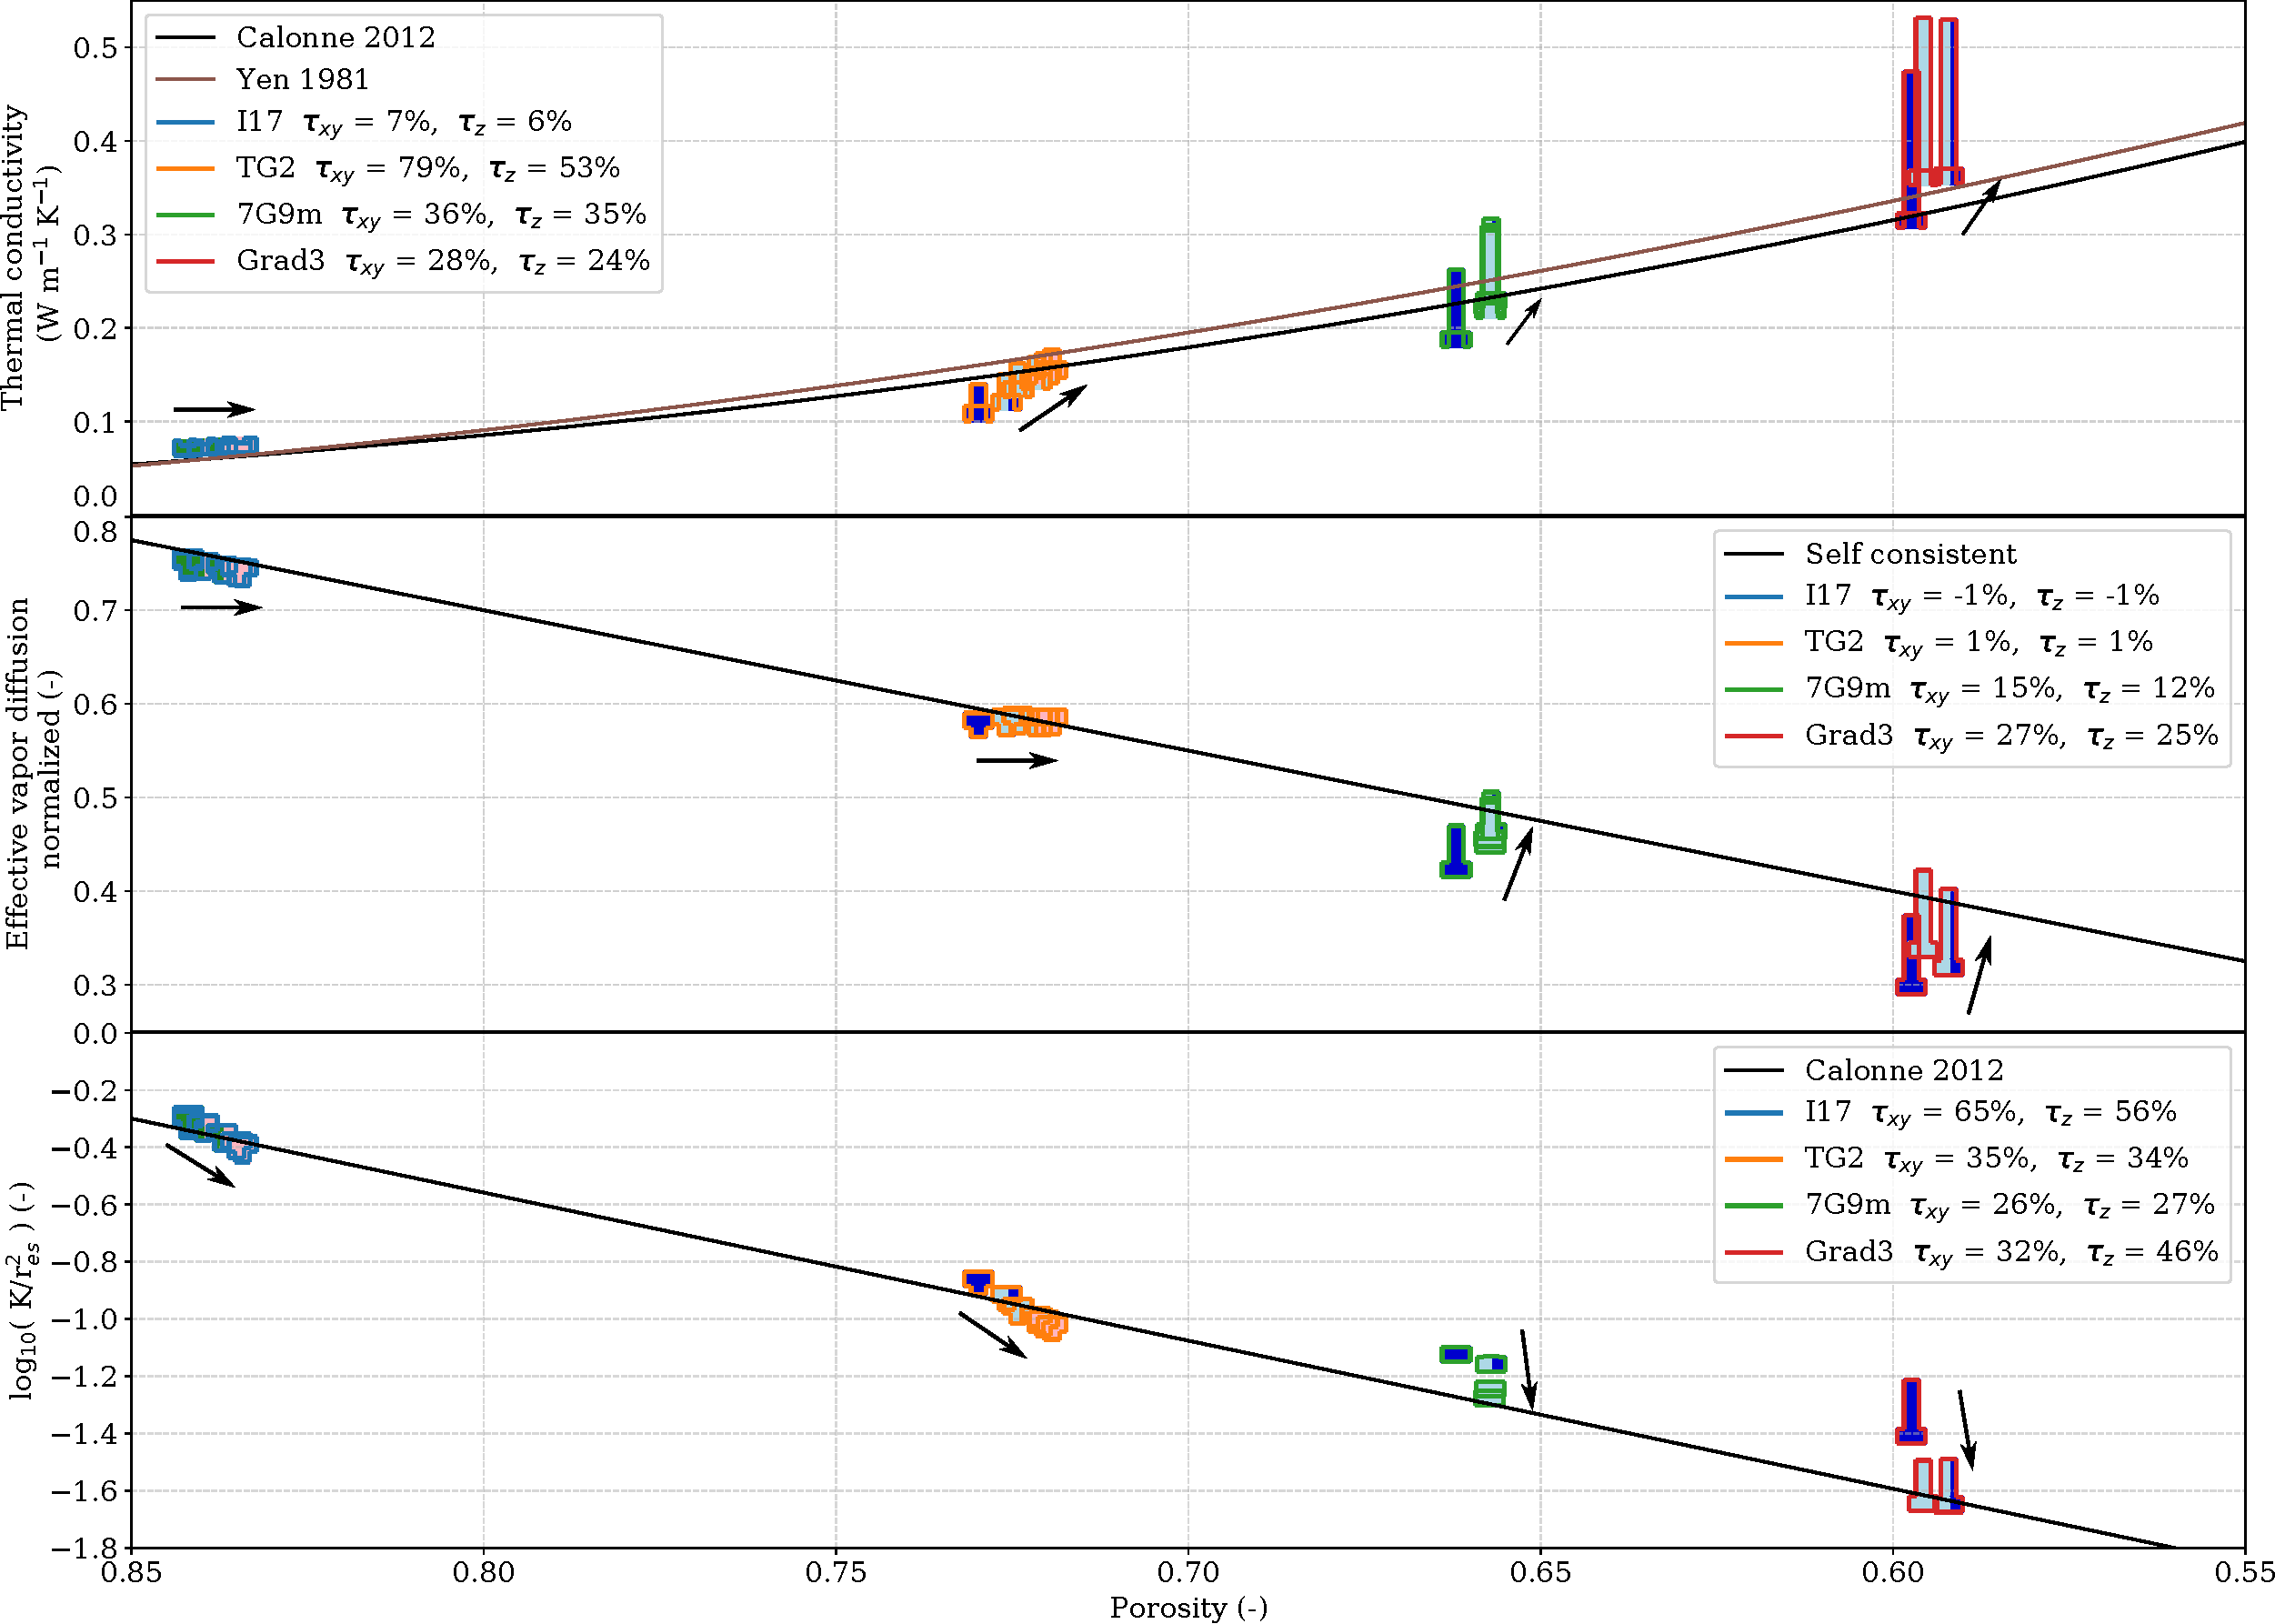
\includegraphics[width=\linewidth]{Figures/Tplot_tau.pdf}
    \caption{Thermal conductivity, normalized vapor diffusion and normalized permeability as a function of porosity.}
    \label{fig:Tplot}
\end{figure}
\section{Discussion}

The main limitation of this study concerns the Snow-3D model and its reliability for modeling isothermal snow metamorphism. The hypotheses of the model are strong and special attention should be given to stay in their extent. The main assumption is related to the physical processes considered in the model. It only computes the sublimation-deposition mechanism, setting other processes potentially occurring in the snow cover aside, in particular grain settling by gravity. The settling process is decisive in the metamorphism of fresh snow, because lots of disconnections occur between the particles at the first stages of metamorphism. Those disconnected ice particles are falling down by gravity in the ice matrix, thus compacting the snow layer. As this effect is not taken into account, one should choose input snow samples that already went through the initial stage of snow compaction. A disconnection correction is applied in the model, it removes ``floating" ice bodies, leading to a loss of mass in the snow volume. This correction was however very small in terms of grain number and mass loss for the studied samples.\\

Another part of the model limitations is the numerical artefacts. The edges of the images are not perfectly simulated due to periodic boundary conditions and the only way to avoid the resulting errors is to analyze the images by removing the borders. This effect can be in contradiction with the REV, which is the minimum size needed to compute parameters. The choice of cutting image edges has only been made for the samples used in the determination of the condensation coefficient $\alpha$, due to the small images used and the precision in SSA and in $\alpha$ needed. To have the maximum precision in all our results, we could have chosen to do so systematically before every property calculation.\\

Another point of interrogation is the time step of the model. The interface width $\varepsilon$, on which the normal vectors are computed, adds a condition on the time step such as $t_{\mathrm{step}} < \varepsilon^2/2$: if the time step exceeds this value, the model will not match the small transformations that should be simulated. Besides this condition we noted an impact of small time steps on the simulation results. This might be due to the edge effect or grid resolution issues.\\

In the computation of microstructural and physical variables, the main limitation is the calculation time. For example, the calculation of permeability can take several days for one image. As a result, we did not analyze a lot of images and only selected the amount of images needed to follow the evolution of the parameters for each series.\\

In the time calibration process, the $\alpha$ parameter has been determined using an experimental series of \citeA{flin_three-dimensional_2004} obtained at -2$^\circ$C. Since $\alpha$ seem to have complex dependency on several parameters, its calibrated value can be influenced by the experimental setup of \citeA{flin_three-dimensional_2004}. To test and validate the calibration, we used the equi-temperature time series of \citeA{hagenmuller_motion_2019}, also realized at -2$^\circ$C. In terms of SSA, the simulated results using the calibrated $\alpha$ and the experimental SSA are in the same order of magnitude, but one can notice that \citeA{hagenmuller_motion_2019} experimental SSA does not follow the decreasing exponential expected curve. As the experimental time series is very short compared to \citeA{flin_three-dimensional_2004}, it can lead to large errors for a longer duration as the given RMSE should be considered dependent on the duration of the series used for the comparison. This impression is however balanced by the comparison of experimental and simulated covariance length, showing a very good fit. It shows that even if the SSA curves does not match, the microstructural evolution under equi-temperature conditions is well simulated.


\section{Conclusion}

The application of \citeA{bretin_phase-field_2019} model to the isothermal metamorphism of snow by the condensation-sublimation process was investigated. The model has been calibrated through the only condensation coefficient $\alpha$ parameter using the SSA of the experimental series of \cite{flin_three-dimensional_2004}. The resulting value is $\alpha = ( 9.92 \pm 0.59) 10^{-4}$. An evaluation of this calibration has been made using the independent experimental series of \cite{hagenmuller_motion_2019} by looking at microstructural properties such as the SSA, the covariance length and the structural anisotropy. As this validation gave very encouraging results, the model Snow3D was used to model isothermal metamorphism on a representative range of microstructures using experimental samples. On the simulated time series, we analyzed microstructural parameters (SSA, $\mathrm{l_{cov}}$, $A_{\mathrm{l_{cov}}}$) and physical transport properties (thermal conductivity, diffusivity and permeability). The comparison of the simulations physical properties and the current related parameterizations shows that the model operates properly for different densities. The microstructural results exhibit the expected global variations for the SSA and covariance length. For the very anisotropic sample Grad3, the structural anisotropy increases with time, leading to a vertical columnar structure. It questions the idea that isotropic conditions could tend to remove the snow structure anisotropy.


\acknowledgments
Enter acknowledgments, including your data availability statement, here.


\bibliography{Snow3D}



%Reference citation instructions and examples:
%
% Please use ONLY \cite and \citeA for reference citations.
% \cite for parenthetical references
% ...as shown in recent studies (Simpson et al., 2019)
% \citeA for in-text citations
% ...Simpson et al. (2019) have shown...
%
%
%...as shown by \citeA{jskilby}.
%...as shown by \citeA{lewin76}, \citeA{carson86}, \citeA{bartoldy02}, and \citeA{rinaldi03}.
%...has been shown \cite{jskilbye}.
%...has been shown \cite{lewin76,carson86,bartoldy02,rinaldi03}.
%... \cite <i.e.>[]{lewin76,carson86,bartoldy02,rinaldi03}.
%...has been shown by \cite <e.g.,>[and others]{lewin76}.
%
% apacite uses < > for prenotes and [ ] for postnotes
% DO NOT use other cite commands (e.g., \citet, \citep, \citeyear, \nocite, \citealp, etc.).
%



\end{document}


